\chapter{Porównanie modeli}
Porównano odpowiedzi obu modeli na skoki wejść do $\pm50\%$ wartości nominalnych. Każda próba rozpoczyna się od podanego punktu równowagi.

\section{Tor sterowania}
\begin{figure}[H]
\centering
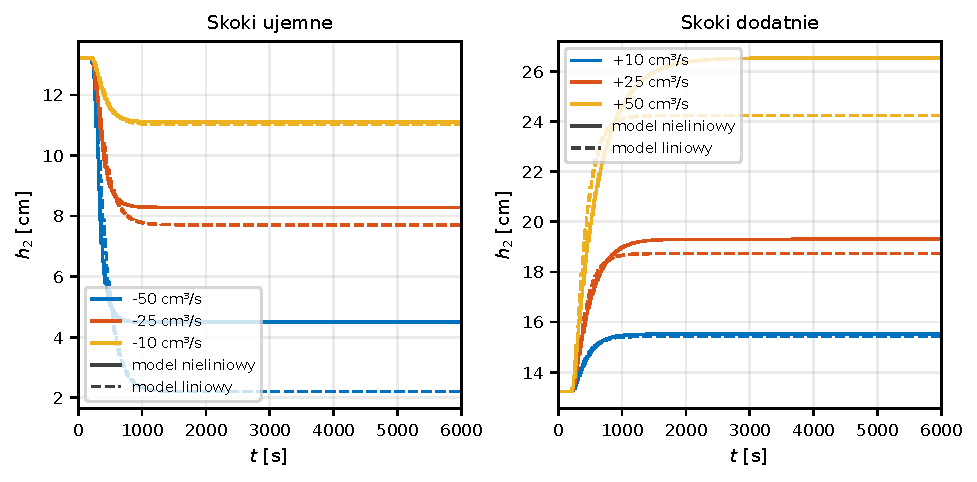
\includegraphics[width=0.90\textwidth]{rysunki/czesc1/skoki_F1in.pdf}
\caption{Skoki sterowania o $\pm10$, $\pm25$ i $\pm50\ \jednprzep$ przy stałym $F_D=20\ \jednprzep$.}
\label{fig:skokiU}
\end{figure}
Blisko punktu pracy odpowiedzi są zbliżone. Dla większych skoków różnią się poziom końcowy i szybkość zmian. Błąd statyczny dla skoków $\pm10\ \jednprzep$ wynosi około $\num{0.092}\ \mathrm{cm}$, a dla $\pm50\ \jednprzep$ około $\num{2.30}\ \mathrm{cm}$.

\section{Tor zakłócenia}
\begin{figure}[H]
\centering
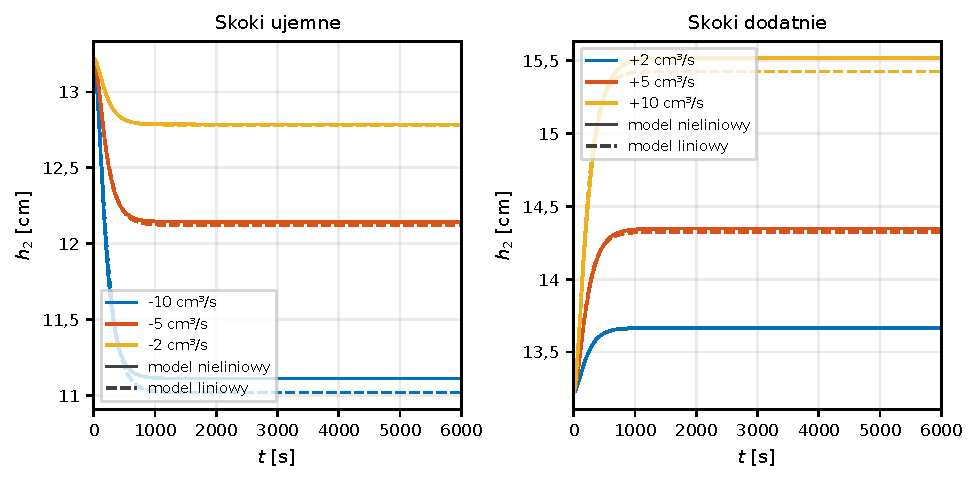
\includegraphics[width=0.90\textwidth]{rysunki/czesc1/skoki_FD.pdf}
\caption{Skoki zakłócenia o $\pm2$, $\pm5$ i $\pm10\ \jednprzep$ przy stałym $\uvar=100\ \jednprzep$.}
\label{fig:skokiD}
\end{figure}
Zakłócenie działa bez opóźnienia transportowego. Różnice modeli są mniejsze, ponieważ skoki $F_D$ mają mniejsze amplitudy bezwzględne niż skoki sterowania.
